\documentclass[10pt]{article}
\usepackage[T1]{fontenc}
\usepackage{lmodern,amsmath,amssymb,graphicx,hyperref}
\usepackage[margin=.72in]{geometry}
\setlength{\parindent}{0pt}\setlength{\parskip}{6pt}
\begin{document}
\begin{center}{\Large Identity origin and public-input cost screen}\\[4pt]
17 November 2026 --- local unsigned Lean evidence\end{center}
\textbf{Constructed identity origin.} On the actual full slot set
$\mathrm{Ports}(a)$ with $u<a$, retain the actual dense integral origin $S$
and its previously constructed inverse. For the same completed matrix $W$
and $D=W_{00}$, set
\[
 K=W+D(S-I),\qquad J=K\,C(S^{-1}).
\]
Local172 constructs the coefficient ring map and derives
$J(0)=I$ from the actual two-sided inverse. At a nonzero source grid node,
$J(t)=W(t)S^{-1}$: these are changed nodes, not the old monomial operators
[pcc:unverified].

\textbf{Whole crossing bound and locality.} Use the unchanged constructed
$m_j=4\,\mathrm{profile}(u,j)$. Let $t\ne0$ be an actual retained integer
node with $v_2(t)=i<u$, let $x_i=y_i$, and let $c_i$ be the old fixed
nonzero diagonalJet. With $\alpha=2^{a+1}$, local173 establishes
\[
 \operatorname{Content}_{u-i}\!\left(c_i^{-1}J_{xy}(t+\alpha Z)\right),
 \qquad
 \operatorname{Content}_{w+u-i}J_{xy}(t+\alpha Z),
 \quad w=\operatorname{jetWeight}(a,u,i,m).
\]
The proof is a finite sum: every nonzero inverse entry preserves the lower
$u$ residue bits, so the old crossing bound applies to each summand;
integrality preserves content under multiplication and summation.
This includes positive anchor zeros and the source root $a=2u$ when $i<u$.
It also derives exact node crossing zeros [pcc:unverified].

Local174 uses actual opposite row/column bit symbols: different groups imply
equal bits and hence zero node entry. A packet-group port subtype has
cardinality at most $2L$. Explicit supplied row/column balance bounds imply
child size at most $6M/r$ and strict eightfold shrink at $r=64$, $M>0$.
Those balance constructors, child tensor identities and entry costs remain
open. Density alone is not an automatic packet-degree failure
[pcc:unverified].

\textbf{Scope of evidence.} Sources172--175 add25 statements to140 accepted
parent statements; final standalone source has165 statements, in addition
to the separately imported base. All four exits are0 with no warnings; every
new dependency print lists only standard foundations. Receipts095--098 and
PCC-20261117-34c9a0, 6d2b50, 205366, 2eb7b3 are unsigned local records,
default \texttt{not\_covered}, outside shared Transport53/57 audit/fresh
[pcc:unverified].

\textbf{Proof map.} Exact declaration endpoints are in
\texttt{INSTANCE-MAP-040.md} through \texttt{043.md} and sources172--175;
receipt artifacts bind source, pre-call, output and exit bytes.
No native identity experiment or performance run was launched.
\newpage
\begin{center}{\Large Screen the actual public-input representation}\end{center}
\textbf{Finite direct-construction bound.} Put every sign bit on one
predicate vertex. Existing actual dummy padding preserves its degree;
it does not split that vertex. Let $b$ be its sign count,
$b\le\Delta$, $u\le a$, $g\ge2$, and $D_{\rm arr}=g^{2a}$.
The primary source D.6 requires
\[
 M\ge 2D_{\rm arr}^{\,2}\Delta.
\]
The square is retained. Natural-power inequalities give
$u\le a\le2^a\le g^a\le D_{\rm arr}\le D_{\rm arr}^2$, and therefore
\[
 bu\le\Delta D_{\rm arr}^2\le M,
 \qquad u>0\Longrightarrow b\le\lfloor M/u\rfloor.
\]
If the field/subgroup bit parameter $n$ is at most $b$, then
$n\le\lfloor M/u\rfloor$ as well. Local175 checks these finite
implications and the actual padded endpoint degree [pcc:unverified].

This screens the direct high-arity parameter certificate. It is not a
runtime lower bound, a statement that all reductions have high degree, or
an exclusion of alternative low-degree representations. The primary
source D.1 uses structural edge parameter $s$ and separate description
length; neither may silently be replaced by ECDLP bit length
[pcc:unverified].

\begin{center}
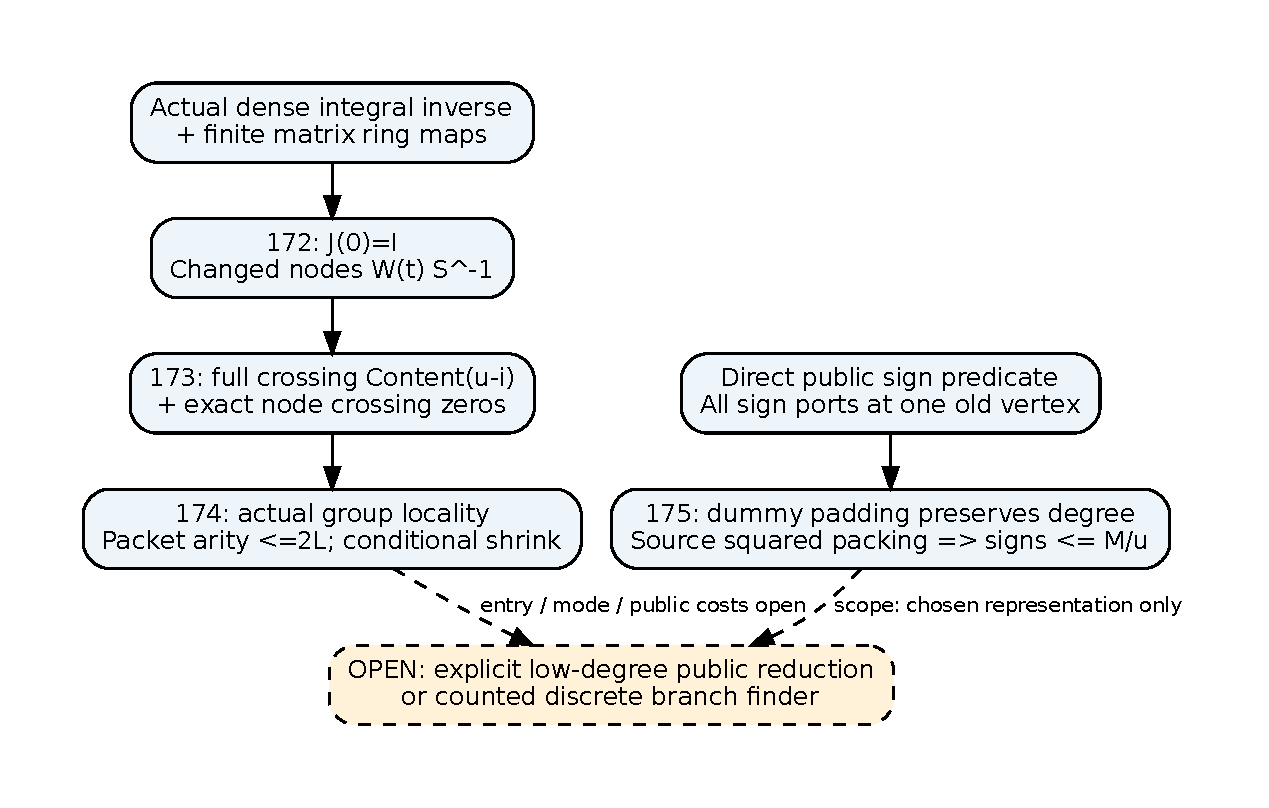
\includegraphics[width=.78\linewidth,height=2.85in,keepaspectratio]{identity-input-dependencies-001.pdf}
\end{center}

\textbf{Next discriminating construction.} Write the actual public
signed-Hankel arithmetic/Boolean network, including shared moments,
bounded-fanout copies, field-bit preparation, entry cost and actual wire
and degree bounds. Test the resulting claimed envelope before more
auxiliary deformation proofs. Alternatively select valid discrete branches
with fewer counted visits; supplied successful signs or continuous repairs
do not discharge that obligation. Original public field/scalar recovery,
retry and expected bit costs remain open.

\textbf{Sources and preservation.} Primary
\texttt{openai-oct25.txt}, D.1/D.4.2/D.4.6; repository
\texttt{NEXT\_FINDER.md} in the prime-norm study; existing Mathlib matrix,
Nat and cardinality laws. KB unavailable; no novelty claim. No speed result
or canonical scoreboard change. Old immutable reports, claims and raw logs
remain exact; this report and diagram are new versioned additions.
\end{document}
